\documentclass[12pt,a4paper]{report}
\usepackage{graphicx}
\usepackage{amsmath}
\usepackage{fancyhdr}
\usepackage{cite}
\usepackage{framed}
\usepackage{a4wide}
\usepackage{float}
\usepackage{epsfig}
\usepackage{longtable}
\usepackage{enumerate}
\usepackage{afterpage}
\usepackage{multirow}
\usepackage{ragged2e}
\usepackage{gensymb}
\usepackage{amsfonts} 
\usepackage[left=3.5cm,top=1.5cm,right=3cm,bottom=4cm]{geometry}
\usepackage{setspace}           
\usepackage{float}
\usepackage{txfonts}
\usepackage{lipsum}

\newcommand{\Usefont}[1]{\fontfamily{#1}\selectfont}

\usepackage{lscape} % for landscape tables
\renewcommand{\baselinestretch}{1.7} 

\usepackage{blindtext}
\usepackage{xpatch}
\usepackage{url}
\usepackage{leqno}
\usepackage{subcaption}

\linespread{1.5}
\usepackage[intoc, english]{nomencl}
\hyphenpenalty=5000
\tolerance=1000
\usepackage[nottoc]{tocbibind}
\bibliographystyle{IEEEtran}
\renewcommand{\bibname}{References}

%*******************************************************************
%                        Header and Footer   
% This is not required in Technical reports submitted to CET ECE department.
% Please leave it commented                       
%*******************************************************************
%\pagestyle{fancy}
%\fancyhead{}
%\header and footer section
%\renewcommand\headrulewidth{0.1pt}
%\fancyhead[L]{\footnotesize \leftmark}
%\fancyhead[R]{\footnotesize \thepage}
%\renewcommand\headrulewidth{0pt}
%\fancyfoot[R]{\small College of Engineering Trivandrum}
%\renewcommand\footrulewidth{0.1pt}
%\fancyfoot[C]{2020 - 2021}
%\fancyfoot[L]{\small Title of the Seminar/Project}
%*******************************************************************


%*********************Figures*****************************
% Save all figures in the folder figures and include them in your 
% report using the command \includegraphics{figure-name}

\graphicspath{{figures/}}

% figure files can be in jpeg,jpg, png or pdf formats
%*******************************************************************


\begin{document}
	
	
%****The entries in this section are to be filled in by the student with appropriate values *************

% These values are used thoroughout the report 
% please fill in the appropriate values

\gdef \title{Constructing an Associative Memory
System Using Spiking Neural
Network} % Seminar title
\gdef \author{SANKAR VINAYAK E P}	 %student name
\gdef \dept{Computer Science and Engineering} %Department
\gdef \degree{Bachelor of Technology} %degree
\gdef \branch{Computer Science and Engineering} %branch
\gdef \college{College of Engineering}
\gdef \collegeplace{Sreekrishnapuram}
\gdef \rollno{PKD19CS046} %KTU Reg No
\gdef \deptabbr{Dept.of CSE} %Dept name abbreviation

\gdef \guide{Liji L Dominic} %Seminar guide
\gdef \guidedes{Assistant Professor}%Seminar guide designation

\gdef \semcordinatorA{Dr. Swaraj K P}% Seminar coordinator 1 
\gdef \semcordinatorAdes{Associate Professor}% Seminar coordinator 1 designation

\gdef \semcordinatorB{Prof. Seminar coordinator 2} % Seminar coordinator 2 
\gdef \semcordinatorBdes{Associate Professor}% Seminar coordinator 2 designation

\gdef \hod{Dr. Sabitha S} %Head of Department
\gdef \hoddes{Professor and Head} %HOD designation

\gdef \acadyear{2022 - 23} % Academic year
\gdef \month{DECEMBER 2022} %Month of Report submission
\gdef \date{15-12-2022} %Date of signing the declaration

%*******************************************************************
% The font pages. The source tex files are there in the folder
%==================================coverpage.tex================================


\newenvironment{coverpage}
\thispagestyle{empty}
\begin{titlepage}
	\begin{center}
		\vspace*{5pt}
		{\Usefont{phv} \Large \bf \title \par}
		\vspace*{20pt}
		\large { 
			A Seminar Report \par
			submitted by\\
		{\bf\author}\\
		{\bf\rollno}\\
			to \\
			the APJ Abdul Kalam Technological University\\
			in partial fulfillment of requirements for the award of degree}\\ [.15\baselineskip] \par of \\
		\Usefont{ppl} {\bfseries  \degree}\\
		in\\
		{\Usefont{ppl} {\bfseries \branch}}\\
		
		\vspace*{30pt}
		\centering
		\begin{figure}[h!]
			\centerline{
\includegraphics[scale=0.4]{logo.png}}
		\end{figure}
		
		\vspace{\stretch{0.5}}
		\footnotesize{\bf DEPARTMENT OF COMPUTER SCIENCE AND ENGINEERING} \par
		\bf{GOVERNMENT ENGINEERING COLLEGE PALAKKAD} \par
		\bf{SREEKRISHNAPURAM 678 633} \par
		\bf{\month}
	\end{center}		
\end{titlepage}	
 %Unless essential Do not edit this tex file



%%********************Certificate*******************

% To print name of only the seminar coordinator 1 in the certificate page
%==================================certificate1.tex================================
% To print name of only the seminar coordinator 1 in the certificate page

\newenvironment{certificate1}

	\newpage
	\begin{center}	
		%\vspace{1.5cm}
		
		\textbf{DEPT. OF COMPUTER SCIENCE ENGINEERING}	
		\textbf{GOVRNMENT ENGINEERING COLLEGE}	
		\textbf{PALAKKAD}
		
		\textbf{\acadyear} 
	\end{center}
	
	
	\begin{center}
		
\includegraphics[scale=0.3]{logo}	
	\end{center}
	\begin{center}
		\textbf{CERTIFICATE}
	\end{center}
	
	This is to certify that the report entitled \textbf{\title} submitted by \textbf{\author}\hspace*{2pt}(\rollno), to the APJ Abdul Kalam Technological University in partial fulfillment of the B.Tech.\ degree in \branch \hspace*{2pt} is a bonafide record of the seminar work carried out by him under our guidance and supervision. This report in any form has not been submitted to any other University or Institute for any purpose.
	
	
	\begin{singlespace}
		\vspace*{1cm}
		\begin{table}[h!]
			\centering
			\begin{tabular}{p{7cm} p{0.9cm} p{7cm}} 
				\textbf{\guide} && \textbf{\semcordinatorA} \\
				(Seminar Guide) &&  (Seminar Coordinator)\\
				\guidedes & & \semcordinatorAdes\\ 
				Dept.of CSE && Dept.of CSE\\ 
				GOVRNMENT ENGINEERING  & &GOVRNMENT ENGINEERING \\
				COLLEGE PALAKKAD && COLLEGE PALAKKAD\\
			\end{tabular}
			
		\end{table}
		
		\vspace*{1.3cm}
		
		\begin{center}
			
			%\hline
			\textbf{\hod} \\ 
			\hoddes\\ 
			Dept.of CSE\\ 
			GOVRNMENT ENGINEERING COLLEGE\\
			PALAKKAD\\
			
		\end{center}
	\end{singlespace}
	
	\thispagestyle{empty}



 

% To print names of both the seminar coordinators in the certificate page
%%==================================certificate2.tex================================
% To print names of both the seminar coordinators in the certificate page
\newenvironment{certificate2}

\newpage
\begin{center}	
	%\vspace{1.5cm}
	
	\textbf{DEPT. OF ELECTRONICS \& COMMUNICATION ENGINEERING}	
	\textbf{COLLEGE OF ENGINEERING}	
	\textbf{TRIVANDRUM}
	
	\textbf{\acadyear} 
\end{center}

\begin{center}
	
\includegraphics[scale=0.5]{cet_logo}	
\end{center}
\begin{center}
	\textbf{CERTIFICATE}
\end{center}

This is to certify that the report entitled \textbf{\title} submitted by \textbf{\author} \hspace*{2pt}(\rollno), to the APJ Abdul Kalam Technological University in partial fulfillment of the B.Tech.\ degree in \branch \hspace*{2pt} is a bonafide record of the seminar work carried out by him under our guidance and supervision. This report in any form has not been submitted to any other University or Institute for any purpose.


\begin{singlespace}
	\vspace*{2cm}
	\begin{table}[h!]
		\centering
		\begin{tabular}{p{7cm} p{0.9cm} p{7cm}} 
			\textbf{\guide} && \textbf{\semcordinatorA} \\
			(Seminar Guide) &&  (Seminar Coordinator)\\
			\guidedes & & \semcordinatorAdes\\ 
			\deptabbr && \deptabbr\\ 
			\college & &\college\\
			\collegeplace && \collegeplace\\
		\end{tabular}
		
	\end{table}
	
	\vspace*{1.3cm}
	
	\begin{center}
		\begin{tabular}{p{7cm} p{0.9cm} p{7cm}} 
			%\hline
			\textbf{\semcordinatorB} && \textbf{\hod} \\
			\semcordinatorBdes & & \hoddes\\ 
			\deptabbr && \deptabbr\\ 
			\college & &\college\\
			\collegeplace && \collegeplace\\
		\end{tabular}
	\end{center}
\end{singlespace}

\thispagestyle{empty}



 %Please uncomment this and comment the previous line

%%***************************************************


%==================================declaration.tex================================
%
\newpage
\newenvironment{declaration}
\thispagestyle{empty}
\chapter*{DECLARATION}
% \begin{center}
%     \vspace*{30pt}
%     \textbf{DECLARATION}\\
% \end{center}
I \author \hspace*{2pt} hereby declare that the seminar report {\bf{\title}}, submitted for partial fulfillment of the requirements for the award of degree of Bachelor of Technology of the APJ Abdul Kalam Technological University, Kerala is a bonafide work done by me under supervision of \guide \hspace*{2pt} \par
This submission represents my ideas in my own words and where ideas or words of
others have been included, I have adequately and accurately cited and
referenced the original sources.\par
I also declare that I have adhered to ethics of academic honesty and integrity
and have not misrepresented or fabricated any data or idea or fact or source in
my submission. I understand that any violation of the above will be a cause for
disciplinary action by the institute and/or the University and can also evoke
penal action from the sources which have thus not been properly cited or from
whom proper permission has not been obtained. This report has not been
previously formed the basis for the award of any degree, diploma or similar
title of any other University.

\noindent \begin{minipage}{0.45\linewidth}
    \begin{flushleft}
        \vspace{4cm}

        \collegeplace \\
        \date

    \end{flushleft}
\end{minipage}
\hfill
\begin{minipage}{0.45\linewidth}
    \begin{flushright}
        \vspace{4cm}

        \author\\

    \end{flushright}
\end{minipage}
\thispagestyle{empty} %Unless essential Do not edit this tex file

\pagenumbering{roman} 

%%********************************Abstract***********************
%============================= abstract.tex================================
\chapter*{\centering Abstract}%
%\addcontentsline{toc}{chapter}{\numberline{}Abstract}%
\begin{center}
    \addcontentsline{toc}{chapter}{Abstract}%
\end{center}

An associative memory system is a type of artificial neural network that can
learn and store associations between input and output patterns. Spiking neural
networks, on the other hand, are a type of neural network that models the
behaviour of neurons in the brain by using discrete time steps to simulate the
firing of individual neurons. Combining these two concepts can result in an
effective memory representation technique in which the contents can be accessed
with speed and efficiency. The report provides an overview of the principles of
associative memory and spiking neural networks, and then describe the
architecture and training procedure for the system. The results show that
spiking neural networks can be effective for implementing associative memory
systems, and have potential applications in a range of computational
neuroscience and machine learning problems.

% The aim of this seminar report is to explore the use of spiking neural networks
% for the construction of associative memory systems. An associative memory
% system is a type of artificial neural network that is able to learn and store
% associations between input and output patterns. Spiking neural networks, on the
% other hand, are a type of neural network that models the behavior of neurons in
% the brain by using discrete time steps to simulate the firing of individual
% neurons. In this report, we will discuss the principles behind both associative
% memory systems and spiking neural networks, and describe how they can be
% combined to create a powerful and efficient associative memory system. We will
% also present some experimental results that demonstrate the effectiveness of
% this approach. Overall, this report presents a promising new approach to the
% construction of associative memory systems, and shows the potential for further
% development and application in a variety of settings.
\begin{flushright}

\end{flushright}

\thispagestyle{plain} % Please type in the abstract in this tex file abstract.tex

%%***************************************************
% Default Acknowledgement page
%==================================acknowledgement.tex=============================
\chapter*{\centering Acknowledgement}%
\addcontentsline{toc}{chapter}{Acknowledgement}%

%\newenvironment{acknowledgement}

I take this opportunity to express my deepest sense of gratitude and sincere
thanks to everyone who helped me to complete this work successfully. I express
my sincere thanks to \textbf{ \hod}, Head of Department, \dept,
\college\hspace*{2pt} \collegeplace \hspace*{2pt} for providing me with all the
necessary facilities and support.\par

I would like to express my sincere gratitude to \textbf{\semcordinatorA} and
\textbf{\semcordinatorB}, \hspace*{2pt} department of \hspace*{2pt} \dept,
\hspace*{2pt} \college \hspace*{2pt} \collegeplace \hspace*{2pt} for their
support and co-operation.

\noindent I would like to place on record my sincere gratitude to my seminar guide \textbf{\guide},\hspace*{2pt}\guidedes,\hspace*{2pt}\dept,\hspace*{2pt}\college \hspace*{2pt} for the guidance and mentorship throughout the course.

Finally I thank my family, and friends who contributed to the succesful
fulfilment of this seminar work.

\vspace*{30pt}
\begin{flushright}
	\textbf{\author}
\end{flushright}
\thispagestyle{plain}  %Unless essential Do not edit this tex file


%%***************************************************
%%**If you have only one seminar coordinator faculty member
% please comment the above line and uncomment this line

%%==================================acknowledgement.tex=============================
\chapter*{Acknowledgement}%
\addcontentsline{toc}{chapter}{Acknowledgement}%

%\newenvironment{acknowledgement}


I take this opportunity to express my deepest sense of gratitude and sincere thanks to everyone who helped me to complete this work successfully. I express my sincere thanks to \textbf{ \hod}, Head of Department, \dept, \college\hspace*{2pt} \collegeplace \hspace*{2pt} for providing  me with all the necessary facilities and support.\par

 I would like to express my sincere gratitude to \textbf{\semcordinatorA}, \hspace*{2pt} department of \hspace*{2pt} \dept, \hspace*{2pt} \college \hspace*{2pt} \collegeplace \hspace*{2pt} for their support and co-operation.

\noindent I would like to place on record my sincere gratitude to my seminar guide \textbf{\guide},\hspace*{2pt}\guidedes,\hspace*{2pt}\dept,\hspace*{2pt}\college \hspace*{2pt} for the guidance and mentorship throughout the course.

Finally I thank my family, and friends who contributed to the succesful fulfilment of this seminar work.

\vspace*{30pt}
\begin{flushright}
	\textbf{\author}
\end{flushright}
\thispagestyle{plain}
  %Unless essential Do not edit this tex file
%*******************************************************************

\thispagestyle{empty}
\newpage
    
%%**********************Table of Contents***********************
\tableofcontents
\listoffigures
\listoftables
%==================================symbol.tex================================
% List of Symbols
\chapter*{List of Symbols}
\addcontentsline{toc}{chapter}{List of Symbols}%
%\makeatletter
%\makeatother
%%\newcommand{\abbrlabel}[1]{\makebox[3cm][l]{\textbf{#1}\ \tocfill}}
\newenvironment{symbols}


% \begin{itemize}	\setlength{\itemsep}{0pt}
% 	\item [$\Omega$] \text{Unit of Resistance}
% 	\item[$\varepsilon^{'}$]  Real part of dielectric constant 
% 	\item[$\mbox{c}$]	Speed of light
% 	\item[$\lambda$]	Wavelength
% 	\item[$\delta$] Delta
% \end{itemize}
		
%\begin{symbols}
%	\item \symbol{$\Omega$} \text{Unit of Resistance}
%	\item \symbol{[$\mu$]} 	\text{Magnetic permeability}
%	\item[$\mu_0$]	Magnetic permeability of free space
%	\item[$\varepsilon$] Relative complex dielectric constant
%	\item[$\varepsilon^{'}$]  Real part of dielectric constant 
%	\item[$\varepsilon^{''}$] Imaginary part of dielectric constant 
%	\item[$\varepsilon_{s}$] Snow surface dielectric constant
%	\item[$\mbox{c}$]	Speed of light
%	\item[$\lambda$]	Wavelength
%	\item[$\tau$] Pulse length of SAR signal
%	\item[$\beta$]  Bandwidth of the SAR signal
%	\item[$\theta$ ] 	Orientation angle 
%	\item[$\theta_{i}$] 	Incidence or local incidence angle
%	\item[$\theta_{r}$]  Local refractive angle 
%	\item[$\delta A$]	Azimuth resolution of the SAR data
%	\item[$L$]    SAR antenna length
%	\item[$\mathbf{E}(\mathbf{r},t)$] Electric field vector
%	\item[$\mathbf{E_{pq}^s}$]	Scattered field vector
%	\item[$\rho(\mathbf{r}, t)$] Volume density of free charges
%	\item[$\mathbf{g}_\mathbf{E}$] Stokes vector


 %List of Symbols (Optional) comment if not required.
% symbold may be added in the file symbol.tex

%%********************Body of the report**********
% Arabic numbering is used in the body of the report

\cleardoublepage
\setcounter{page}{1}
\pagenumbering{arabic}

%%********************Chapter 1**********
\chapter{Introduction}
\lipsum[1] % Please comment this line and type in the introduction chapter

%%********************Chapter 2**********
\chapter{Literature Review}
Technical writing is writing or drafting technical communication used in technical and occupational fields\cite{india}, such as computer hardware and software\cite{rpi}, engineering, chemistry, aeronautics, robotics, finance\cite{japan}, medical, consumer electronics, biotechnology, and forestry. Technical writing encompasses the largest sub-field in technical communication. See figure \ref{net2} that shows the autonomous systems in Internet.

\begin{figure}[h!]
	\centering
	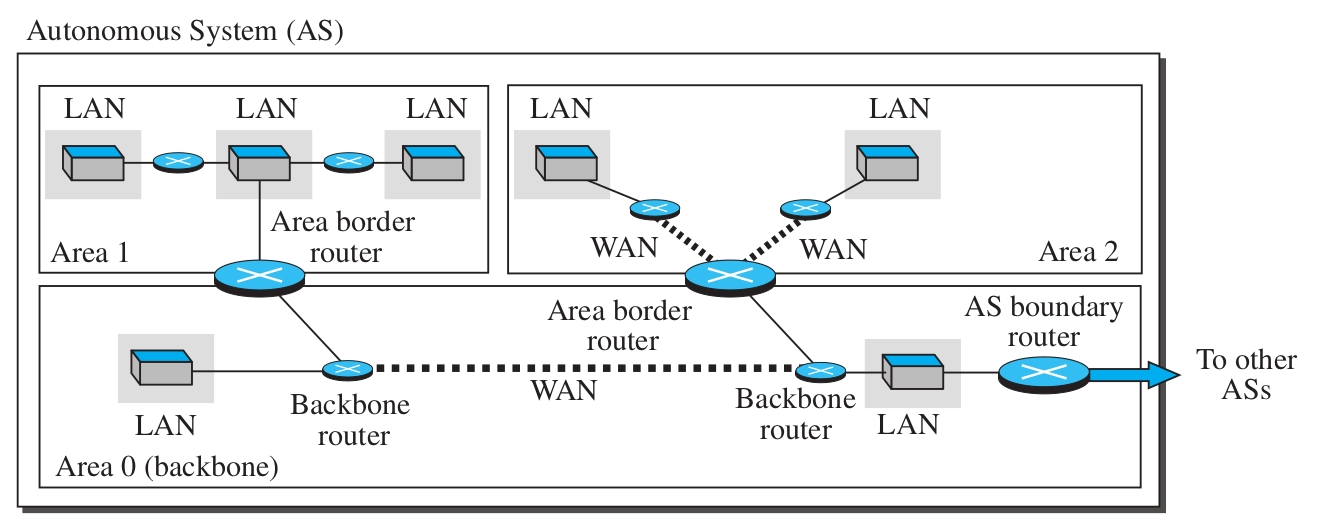
\includegraphics[width=0.9\linewidth]{ospf}
	\caption{Autonomous System Hierarchy}
	\label{net2}
\end{figure}

\section{section1}
\lipsum[2] % Please comment this line and type in the introduction chapter


\subsection{title 2}
\lipsum[3] % Please comment this line and type in the introduction chapter

\noindent The system is described by the equation \ref{sys_eq1} below. Here y is the ordinate and x is the abscissa , m is the slope and c a constant.

\begin{equation} \label{sys_eq1}
y = mx + c
\end{equation}
\noindent Page centered and unnumbered multiple equations. The * symbol supresses equation numbering.
% Page centered and unnumbered equations
\begin{align*}
2x - 5y &=  8 \\ 
3x + 9y &=  -12
\end{align*}

\noindent Side by side figures can be created using this environment. See fig \ref{wave} below.
\begin{figure}[h!]
	\centering
	\begin{subfigure}[b]{0.4\textwidth}
		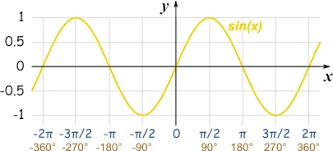
\includegraphics[width=\textwidth]{sinewave}
		\caption{Sine Wave}
		\label{fig:1}
	\end{subfigure}
	\hspace{20mm}
	\begin{subfigure}[b]{0.4\textwidth}
		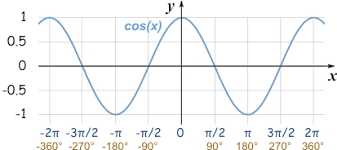
\includegraphics[width=\linewidth]{cosine}
		\caption{Cosine Wave}
		\label{fig:2}
	\end{subfigure}
\caption{The Sine and Cosine waves}
\label{wave}
\end{figure}

%%********************Chapter 3**********
\chapter{Results}
\lipsum[5-7] % Please comment this line and type in the results chapter
	
\begin{table}[h!]
	\centering
	\caption{test table}
	\vspace*{5pt}
	\begin{tabular}{|c|c|c|}
		\hline
		Sl. No & Item 1 & Itm 2 \\ \hline
		1      & 37     & 45    \\ \hline
		2      & 42     & 23    \\ \hline
		3      & 47     & 1     \\ \hline
		4      & 52     & -21   \\ \hline
		5      & 57     & -43   \\ \hline
		6      & 62     & -65   \\ \hline
		7      & 67     & -87   \\ \hline
		8      & 72     & -109  \\ \hline
		9      & 77     & -131  \\ \hline
		10     & 82     & -153  \\ \hline
	\end{tabular}
\end{table}

%%********************Chapter 4**********
\chapter{Conclusion}
\lipsum[2] 

%%********************References**********
%%****This template uses IEEE bibliography style

 \begin{thebibliography}{99}
	\bibitem{india} HU, Yun Chao, et al., \emph{Mobile edge computing?A key technology
		towards 5G}, ETSI white paper, 2015, vol. 11, no 11, p. 1-16.
	
	
	\bibitem{rpi}
	@online{ Raspberry pi,
		\url{https://www.raspberrypi.org/}
		Online; accessed 10-June-2019
	}
	
	\bibitem{japan} HU, Yun Chao, et al., \emph{Mobile edge computing?A key technology
		towards 5G}, ETSI white paper, 2015, vol. 11, no 11, p. 1-16.		
\end{thebibliography}

\end{document}